% xelatex - bibtex - xelatex - xelatex

\documentclass[UTF8]{ctexart}

% 调整版式,减少页边距
\usepackage[top=1.2in,bottom=1.2in,left=1.2in,right=1.2in]{geometry}

% 超链接
\usepackage{color}
\usepackage{hyperref}
\hypersetup{colorlinks=true, linkcolor=blue,  anchorcolor=blue,  
citecolor=blue, filecolor=blue, menucolor=blue, urlcolor=blue}

% 新定义一个命令,方便在正文中使用一些类名、变量名等
\setmonofont{Courier New}
\newcommand{\code}{\texttt}

% C++源代码
\usepackage{listings}
\lstset{
	language=[Visual]C++,
	keywordstyle=\bfseries\ttfamily\color[rgb]{0,0,1},
	identifierstyle=\ttfamily,
	commentstyle=\color[rgb]{0.133,0.545,0.133},
	stringstyle=\ttfamily\color[rgb]{0.627,0.126,0.941},
	showstringspaces=false,
	basicstyle=\ttfamily\small,
	numberstyle=\footnotesize,
	numbers=left,
	stepnumber=1,
	numbersep=10pt,
	tabsize=4,
	breaklines=true,
	prebreak = \raisebox{0ex}[0ex][0ex]{\ensuremath{\hookleftarrow}},
	breakatwhitespace=false,
	aboveskip={0.5\baselineskip},
    belowskip={0.5\baselineskip},
	columns=fixed,
	upquote=true,
	extendedchars=true,
	frame=tb,
	% backgroundcolor=\color{lbcolor},
	% escapeinside=``, % 处理过长的中文注释
    xleftmargin=2em,
    %xrightmargin=2em,
}

% 改变section title的对齐方式
\usepackage{sectsty}
\allsectionsfont{\raggedright} % 左对齐

% 改变title, author, date的对齐方式
\usepackage{titling}

% 图片
\usepackage{graphicx}

\begin{document}

\title{English Title \\中文标题}
\author{作者}
\date{\today}

\pretitle{\begin{flushleft}\heiti \huge} \posttitle{\end{flushleft}}
\preauthor{\begin{flushright}\heiti} \postauthor{\end{flushright}}
\predate{\begin{flushright}\heiti}\postdate{\end{flushright}}
\maketitle

正文。引用\cite{Box1998}。节\ref{sec:fig}。图\ref{fig:demo}。

English text. Class \code{Time}.

\section{图片示例}\label{sec:fig}

\begin{figure}[htbp]
\centering
\label{fig:demo}
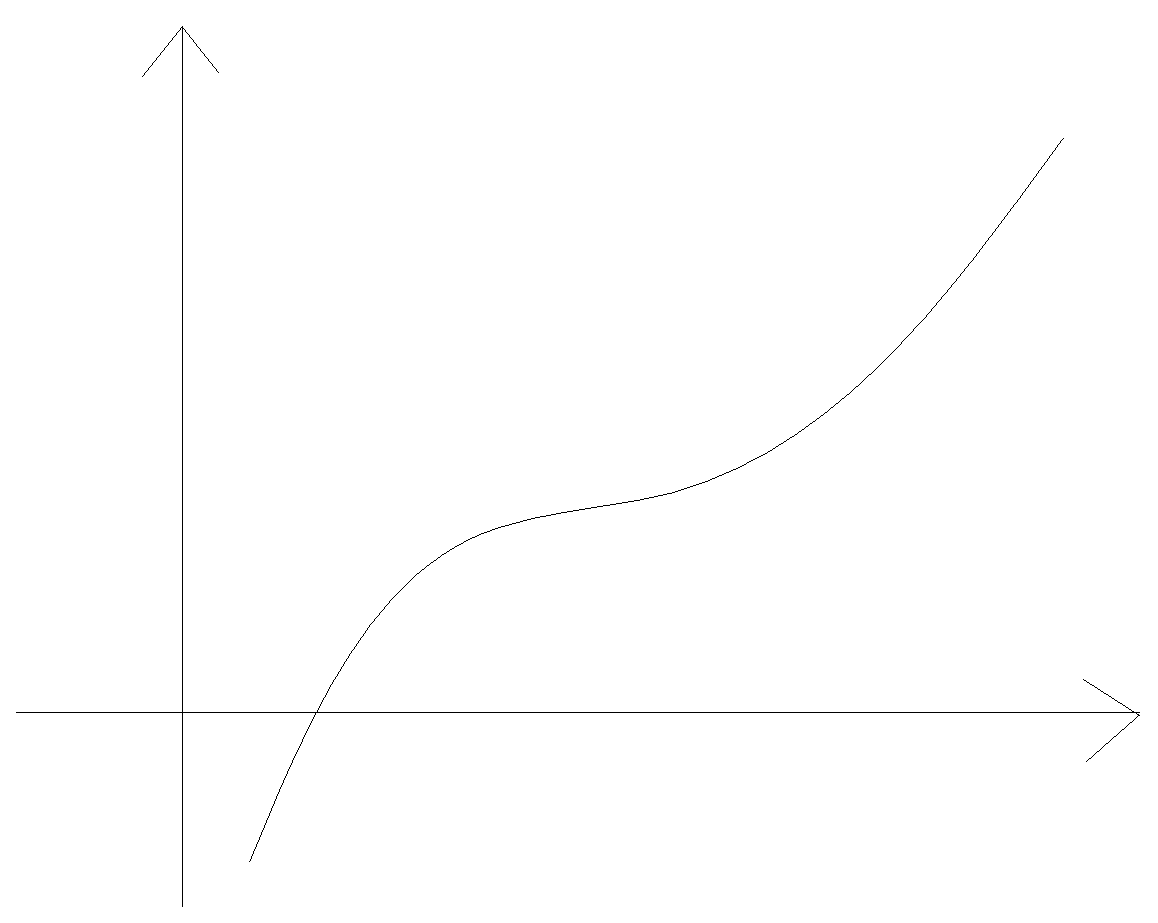
\includegraphics[scale=0.25]{figures/fig32a}
\caption{Demo.}
\end{figure}

\section{公式示例}
$$y = \sin \frac{x}{a}$$

\section{源代码示例}

\begin{lstlisting}
// header: <ctime>
time_t systemTime = time(0);
printf("The Current System Time is \%s", ctime(&systemTime));
\end{lstlisting}

\bibliographystyle{plain}
\bibliography{refs}

\end{document}